\section{Introduction}
Over the past two decades, major advances have been made in estimating structured parameters, e.g., sparse, low-rank, etc., in high-dimensional small sample problems \cite{donoho2006compressed,candes2010power,friedman2008sparse}. Such estimators consider a suitable (semi) parametric model of the response: $y = \phi(\x,\bbeta^*) + \omega$ based on $n$ samples $\{(\x_i,y_i)\}_{i=1}^n$ and $\bbeta \in \reals^p$ is the parameter of interest. The unique aspect of such high-dimensional setup is that the number of samples $n < p$, and the structure in $\bbeta^*$, e.g., sparsity, low-rank, makes the estimation possible \cite{tibshirani1996regression,candes2006robust,candes2009exact}. In several real world problems, natural grouping among samples arises and learning a single global model $\bbeta_0$ for all samples or many local model $\bbeta_g$ per group are unrealistic. The middle ground model for such a scenario is the \emph{superposition} of global and local parameters $\bbeta_0 + \bbeta_g$ which has been of recent interest in the statistical machine learning community \cite{guba16} and is known by multiple names. It is a form of multi-task learning \cite{Zhang2017-rm, jrsr10} when you consider regression in each group as a task. It is also called data sharing \cite{grti16} since information contained in different group is shared through the common parameter $\bbeta_0$. And finally, it has been called data enrichment \cite{Chen2015-fj, Asiaee2018-eg} because we enrich our data set with pooling multiple samples from different but related data sources.


In this paper, we consider the following \emph{data enrichment} (DE) linear model where there is a \emph{common} parameter $\bbeta^*_0$ shared between all groups plus \emph{individual} per-group parameters $\bbeta_g^*$ which characterize the deviation of group $g$, i.e.,
\be
\label{eq:dsl}
y_{gi} = \phi(\x_{gi}, (\bbeta_0^* + \bbeta^*_g)) + \omega_{gi}, \quad g \in \{1, \dots, G\},
\ee
where $g$ and $i$ index the group and samples respectively. %, Figure \ref{fig:cat}. 
Note that the DE model is \emph{a system of coupled superposition models}.
We specifically focus on the high-dimensional small sample regime for \eqref{eq:dsl} where the number of samples $n_g$ for each group is much smaller than the ambient dimensionality, i.e., $\forall g: n_g \ll p$. Similar to all other high-dimensional models, we assume that the parameters $\bbeta_g$ are structured, i.e., for suitable convex functions $f_g$'s, $f_g(\bbeta_g)$ is small. Further, for the technical analysis and proofs,
we focus on the case of linear models, i.e., $\phi(\x,\bbeta) = \x^T \bbeta$. The results seamlessly extend to more general non-linear models, e.g., generalized linear models, broad families of semi-parametric and single-index models, non-convex models, etc., using existing results, i.e., how models like Lasso have been extended to these settings. %(e.g.~employing ideas such as restricted strong convexity \cite{negahban2012restricted}). 

In the context of MTL, similar models have been proposed which has the general form of $y_{gi} = \x_{gi}^T (\bbeta_{1g}^* + \bbeta^*_{2g}) + \omega_{gi}$ where $\B_1 = [\bbeta_{11}, \dots, \bbeta_{1G}]$ and $\B_2 = [\bbeta_{21}, \dots, \bbeta_{2G}]$ are two parameter matrices \cite{Zhang2017-rm}. To capture relation of tasks, different types of constraints are assumed for parameter matrices. For example, \cite{Chen2012-fb} assumes $\B_1$ and $\B_2$ are sparse and low rank respectively. In this parameter matrix decomposition framework for MLT, the most related work to ours is the one proposed by \cite{jrsr10} where authors regularize the regression with $\norm{\B_1}{1, \infty}$ and $\norm{\B_2}{1,1}$ where norms are $p,q$-norms on rows of matrices. Parameters of $\B_1$ are more general than DE's common parameter when we use  $f_0(\bbeta_0) = \norm{\bbeta_0}{1}$. This is because $\norm{\B_1}{1, \infty}$ regularizer enforces shared support of $\bbeta^*_{1g}$s, i.e., $\text{supp}(\bbeta_{1i}^*) = \text{supp}(\bbeta_{1j}^*)$ but allows $\bbeta_{1i}^* \neq \bbeta_{1j}^*$. Further sparse variation between parameters of different tasks is induced by $\norm{\B_2}{1,1}$ which has  a similar effect of DE's individual parameters where $f_g(\cdot)$s are $l_1$-norm. Our analysis of DE framework suggests that it is more data efficient than this setup of \cite{jrsr10} because they require every task $i$ to have large enough samples to learn its own common parameters $\bbeta_i$ while DE shares the common parameter and only requires the {\em{total dataset over all tasks}} to be sufficiently large.

%\ab{need a line on what Jalali et al.~show, and how our results are (qualitatively) different} 
%\ab{we don't have a discussion on `related work' -- including hierarchical models, multi-task learning; should we have a sub-section on these, or otherwise discuss these related developments}
%Also \cite{jrsr10} considers only the cases where function $f_g(\cdot)$ are $l_1$-norm.
%At a high level, the DE model can be viewed as a
%of hierarchical additive model \cite{hastie2017generalized,rigby2005generalized} {\color{red}{couldn't find good ref, we might want to remove this}}, where $\bbeta_0^*$ corresponds to the root and $\bbeta_g^*$ correspond to the refinements in the leaves. 


The DE model where $\bbeta_g$'s are sparse has recently gained attention because of its application in wide range of domains such as personalized medicine \cite{domu16}, sentiment analysis, banking strategy \cite{grti16}, single cell data analysis \cite{olvi15}, road safety \cite{olvi14}, and disease subtype analysis \cite{domu16}.
%More generally, in any high-dimensional problem where the population consists of groups, data enrichment framework has the potential to boost the prediction accuracy and results in a more interpretable set of parameters.
In spite of the recent surge in applying data enrichment framework to different domains, limited advances have been made in
understanding the statistical and computational properties of suitable estimators for the data enriched model.
In fact, non-asymptotic statistical properties, including sample complexity and statistical rates of convergence, of regularized estimators for the data enriched model is still an open question \cite{grti16, olvi14}.
To the best of our knowledge, the only theoretical guarantee for data enrichment is provided in \cite{olvi15} where authors prove sparsistency of their proposed method under the stringent irrepresentability condition of the design matrix for recovering supports of common and individual parameters.
%\ab{If they show support recovery, the condition may have been necessary -- maybe give them due credit, and show how much more the current results are, though we are doing norm consistency, not support recovery.}
Existing support recovery guarantees \cite{olvi15} and sample complexity and $l_2$ consistency results \cite{jrsr10} of related models are restricted to sparsity and $l_1$-norm, while our estimator and \emph{norm consistency} analysis work for any structure induced by arbitrary convex functions $f_g$. 
Moreover, no computational results, such as rates of convergence of the optimization algorithms associated with proposed estimators, exist in the literature.
%{\color{red} TODO: Emphasis that functions can be non-convex.}

%\newlength\heightfiga\newlength\heightcapa
%\newlength\heightfigb\newlength\heightcapb
%\newlength\heightfigc\newlength\heightcapc
%\newlength\heightfig
%
%\begin{figure*}
%	%Definition of lengths
%	\setlength\heightfiga{3cm}
%	\setlength\heightfigb{3cm}
%	\setlength\heightcapa{1\baselineskip}
%	\setlength\heightcapb{2\baselineskip}
%	%Do not change
%	\setlength\heightcapc{\heightcapa}
%	\setlength\heightfigc{\heightfiga+\heightfigb+\heightcapa}
%	\setlength\heightfig{\heightfigc+\heightcapc}
%	\begin{minipage}[b][\heightfig][t]{0.68\linewidth}
%		\centering
%		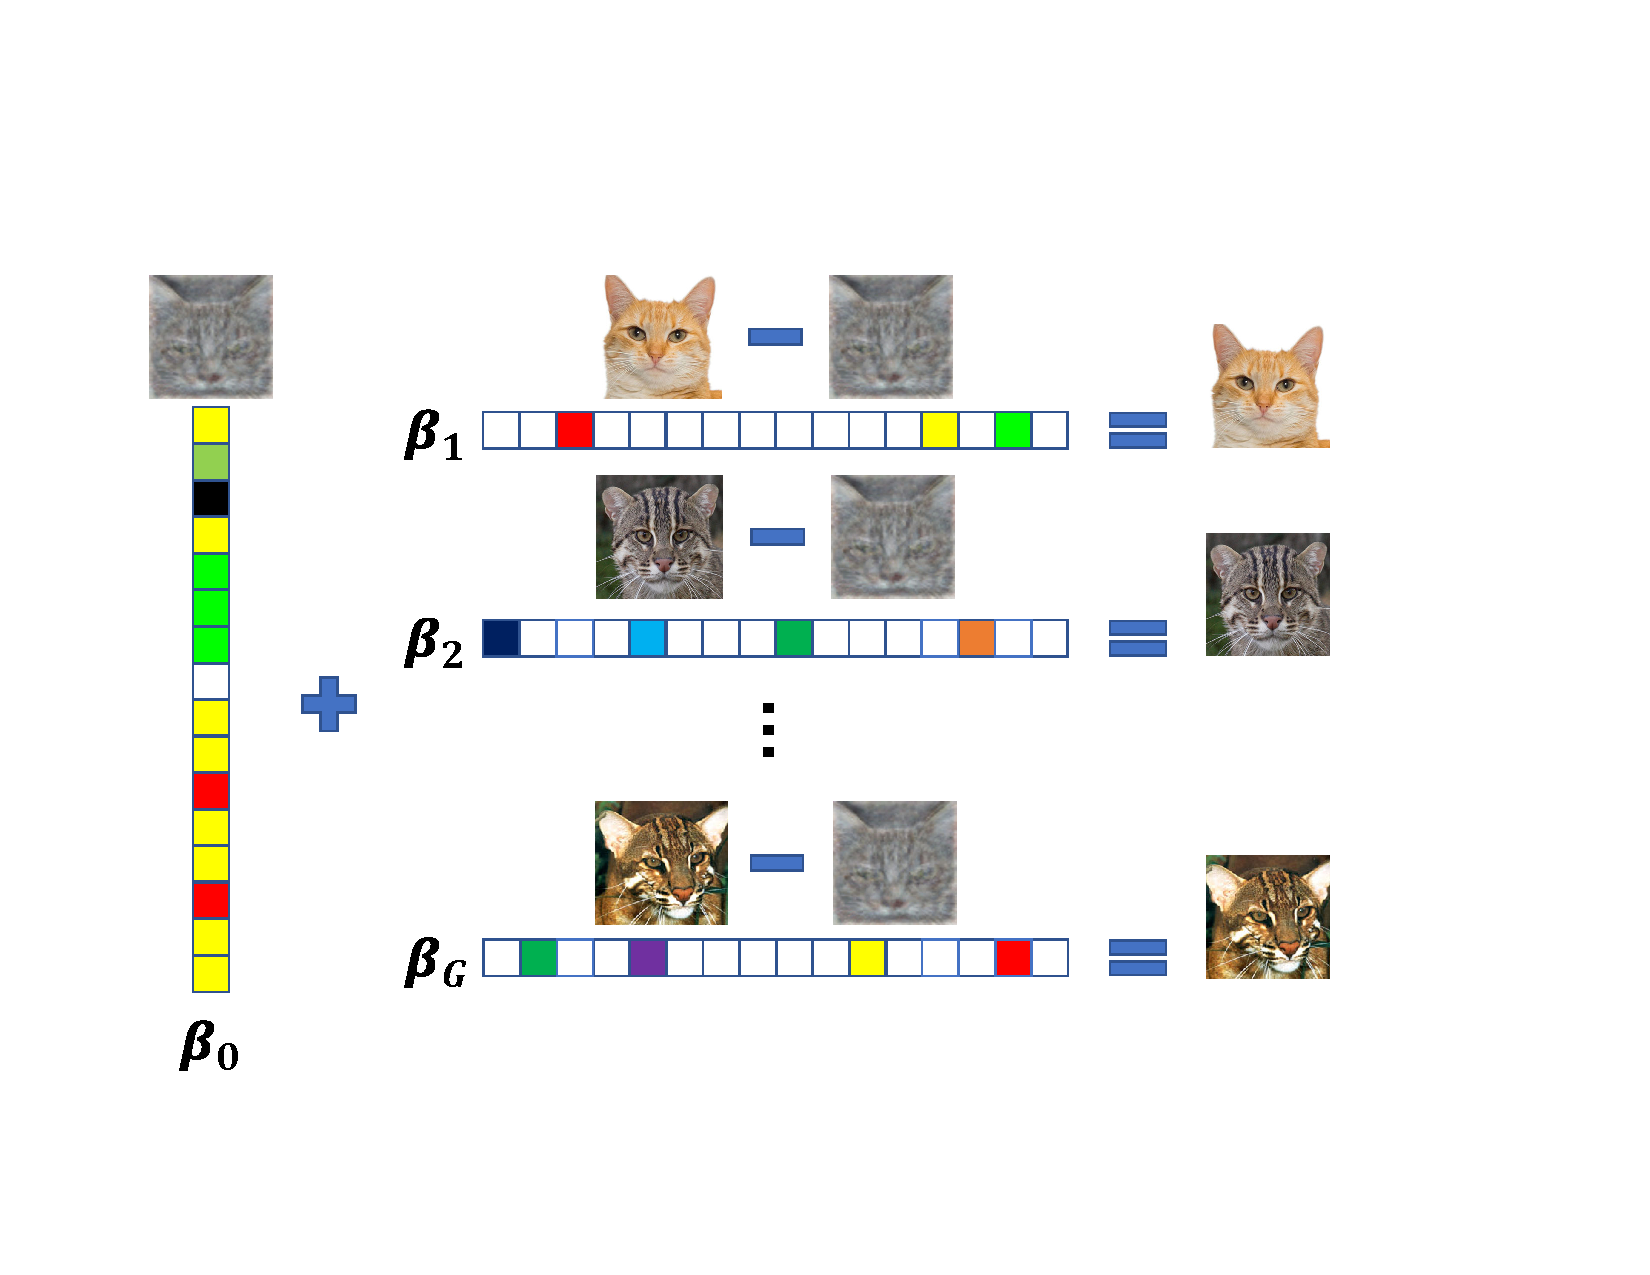
\includegraphics[height=\heightfigc]{./img/concept}
%		\parbox[b][\heightcapc][t]{1.\linewidth}{\subcaption{Data Enrichment.}\label{subfig3}}
%	\end{minipage}	\hfill
%	\begin{minipage}[b][\heightfig][t]{0.3\linewidth}\centering
%		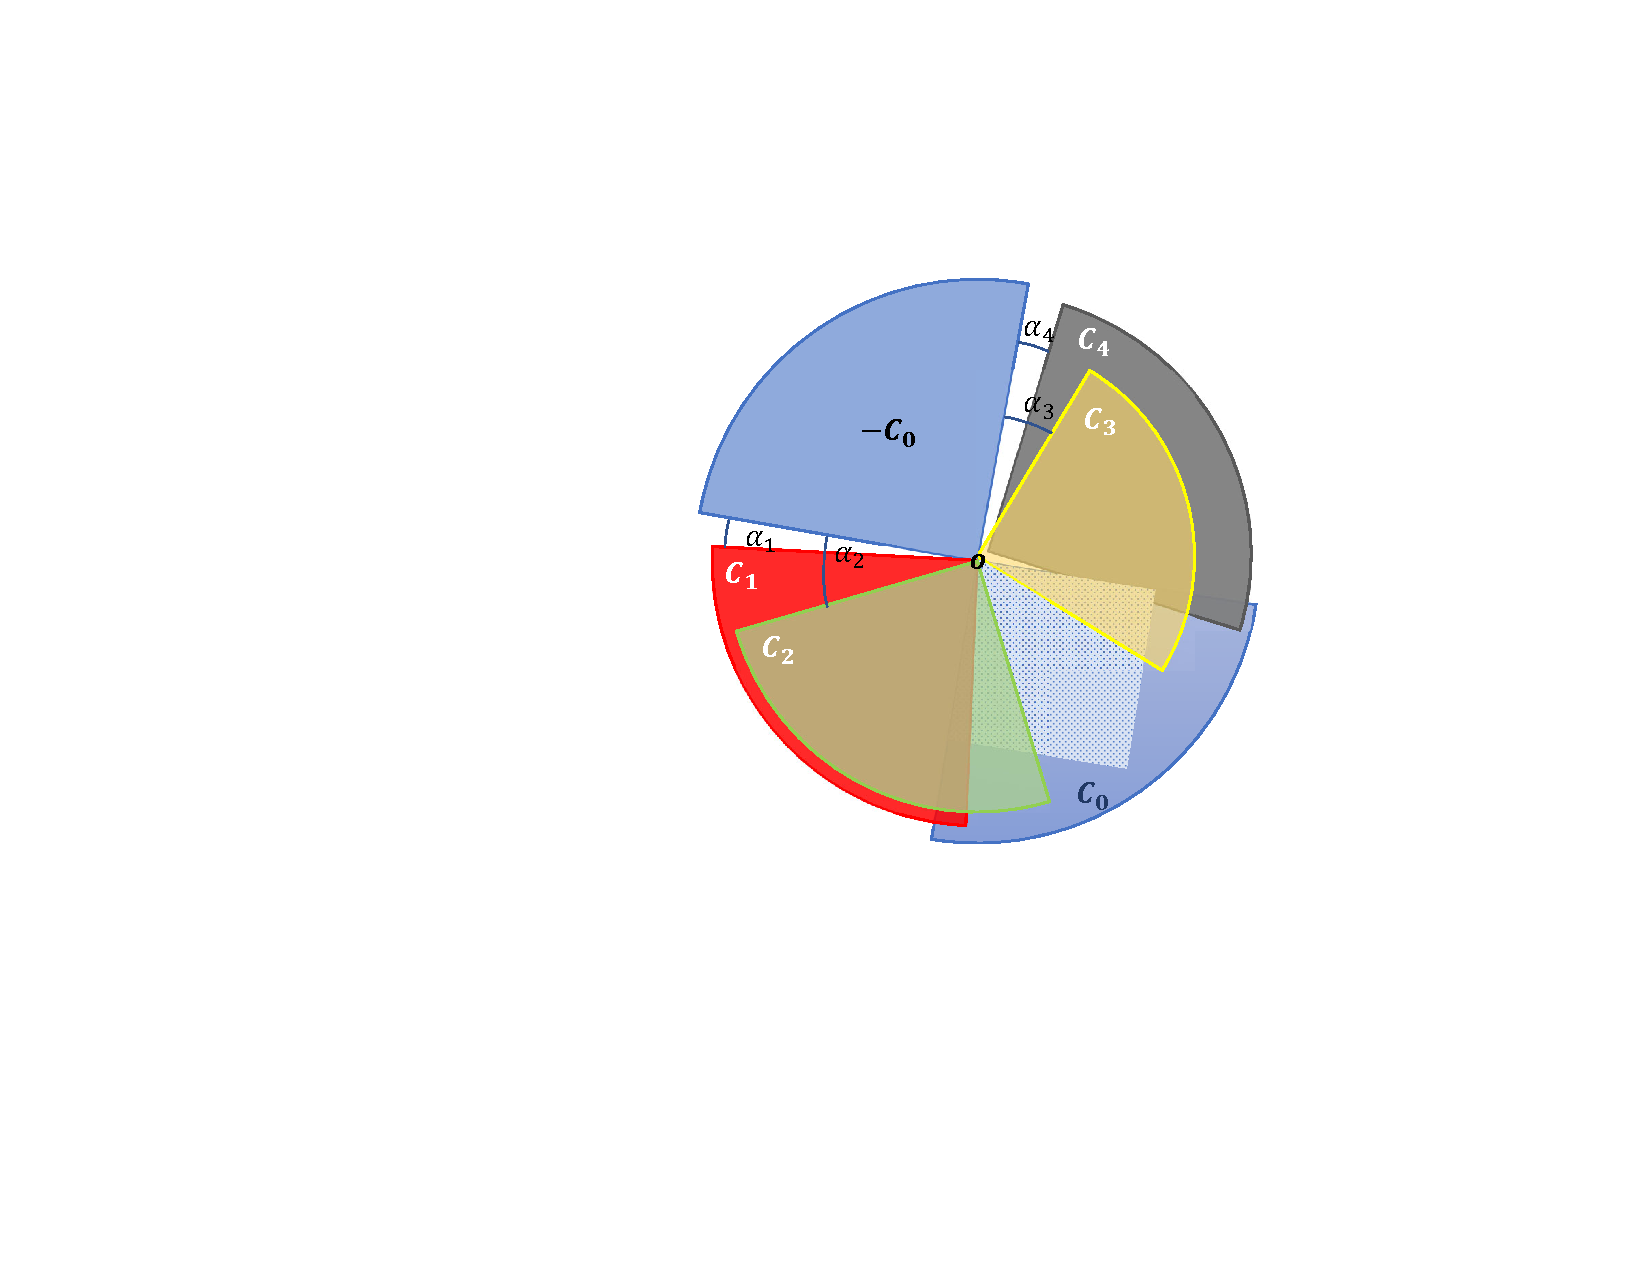
\includegraphics[height=\heightfiga]{./img/sc.pdf}
%		\parbox[b][\heightcapa][t]{1\linewidth}{\subcaption{SC}\label{subfig1}}
%		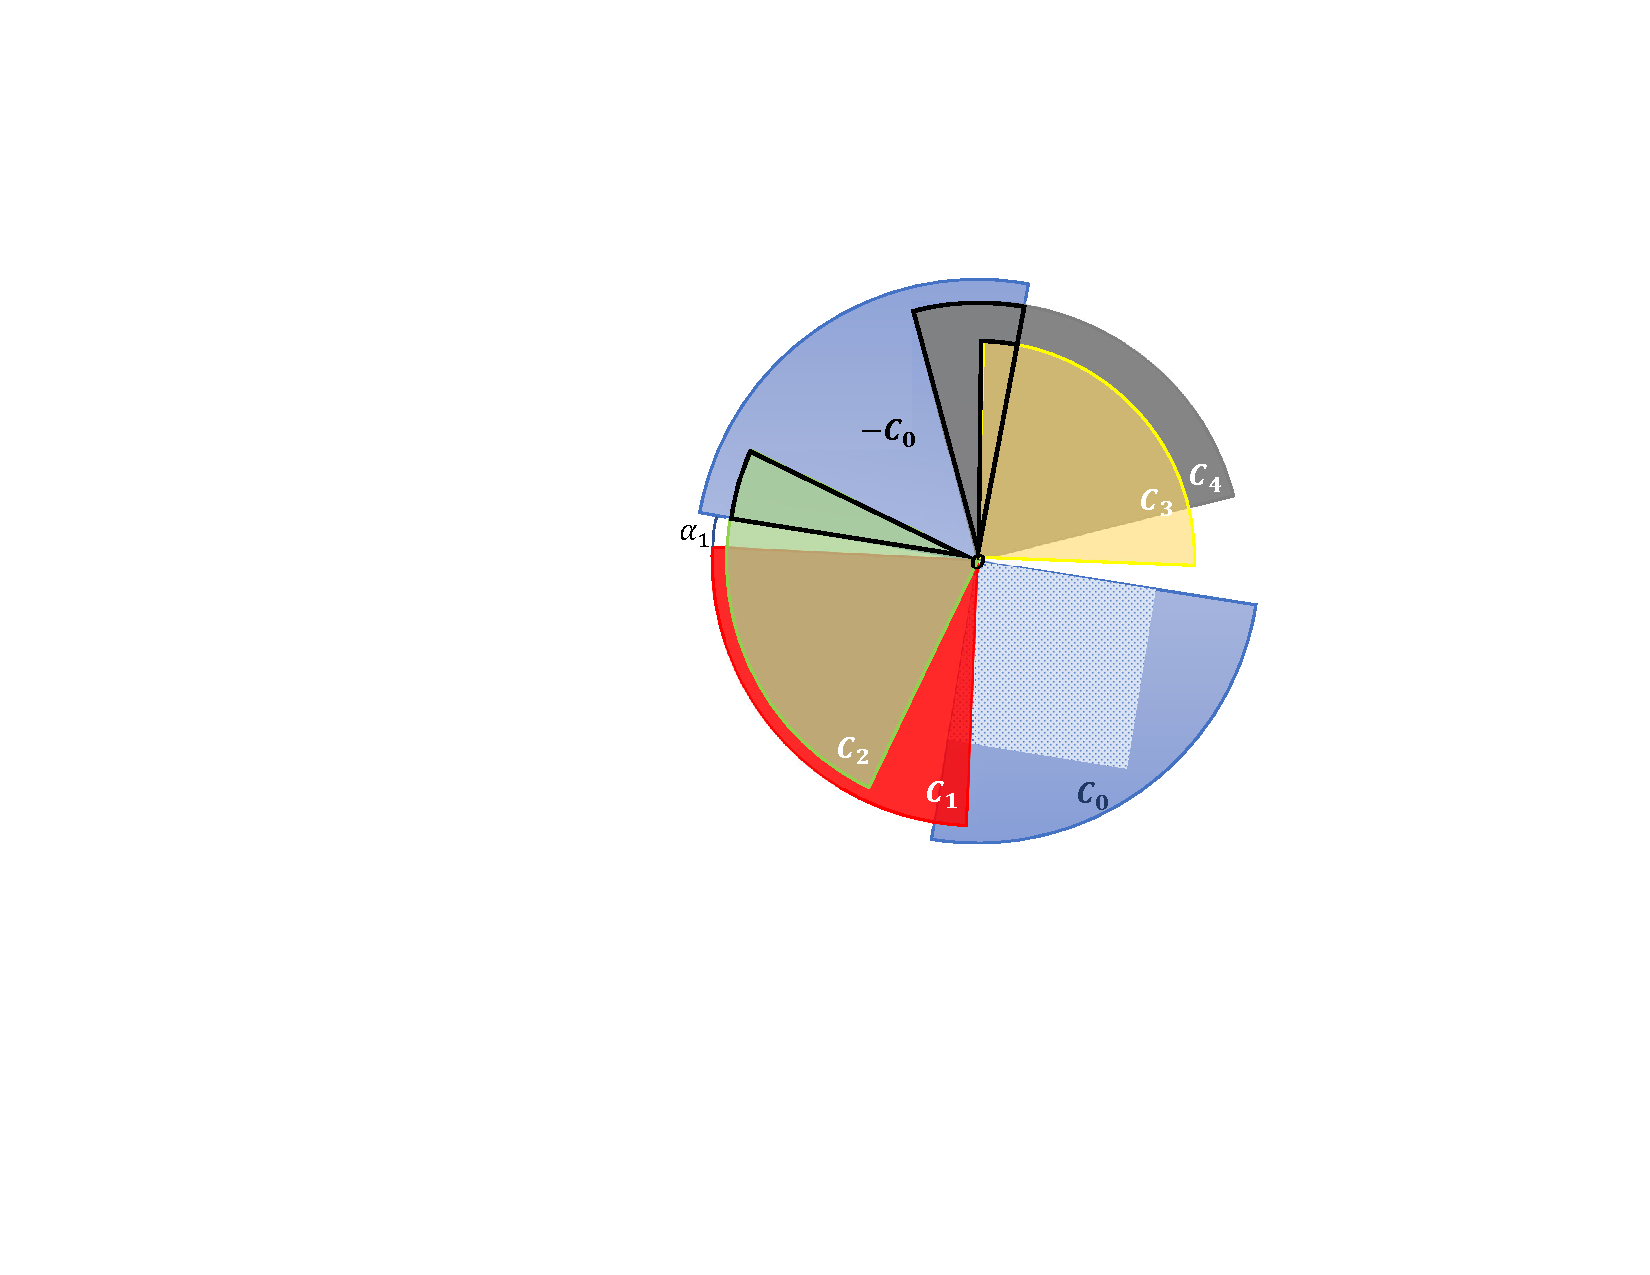
\includegraphics[height=\heightfigb]{./img/deric.pdf}
%		\parbox[b][\heightcapb][t]{1\linewidth}{\subcaption{DERIC}\label{subfig2}}
%	\end{minipage}
%	\caption{a) A conceptual illustration of data enrichment model for learning representation of  different cat species. The common parameter $\bbeta_0$ captures a \emph{generic cat} which consists of shared features among all cats. b) Our  c) Distribution of responses to Saracatinib. Note that some cell lines of both lung and blood cancers have responded to Saracatinib which makes it a good candidate for interpretability analysis.}
%	\label{fig}
%\end{figure*}
%\begin{figure}
%		\centering
%		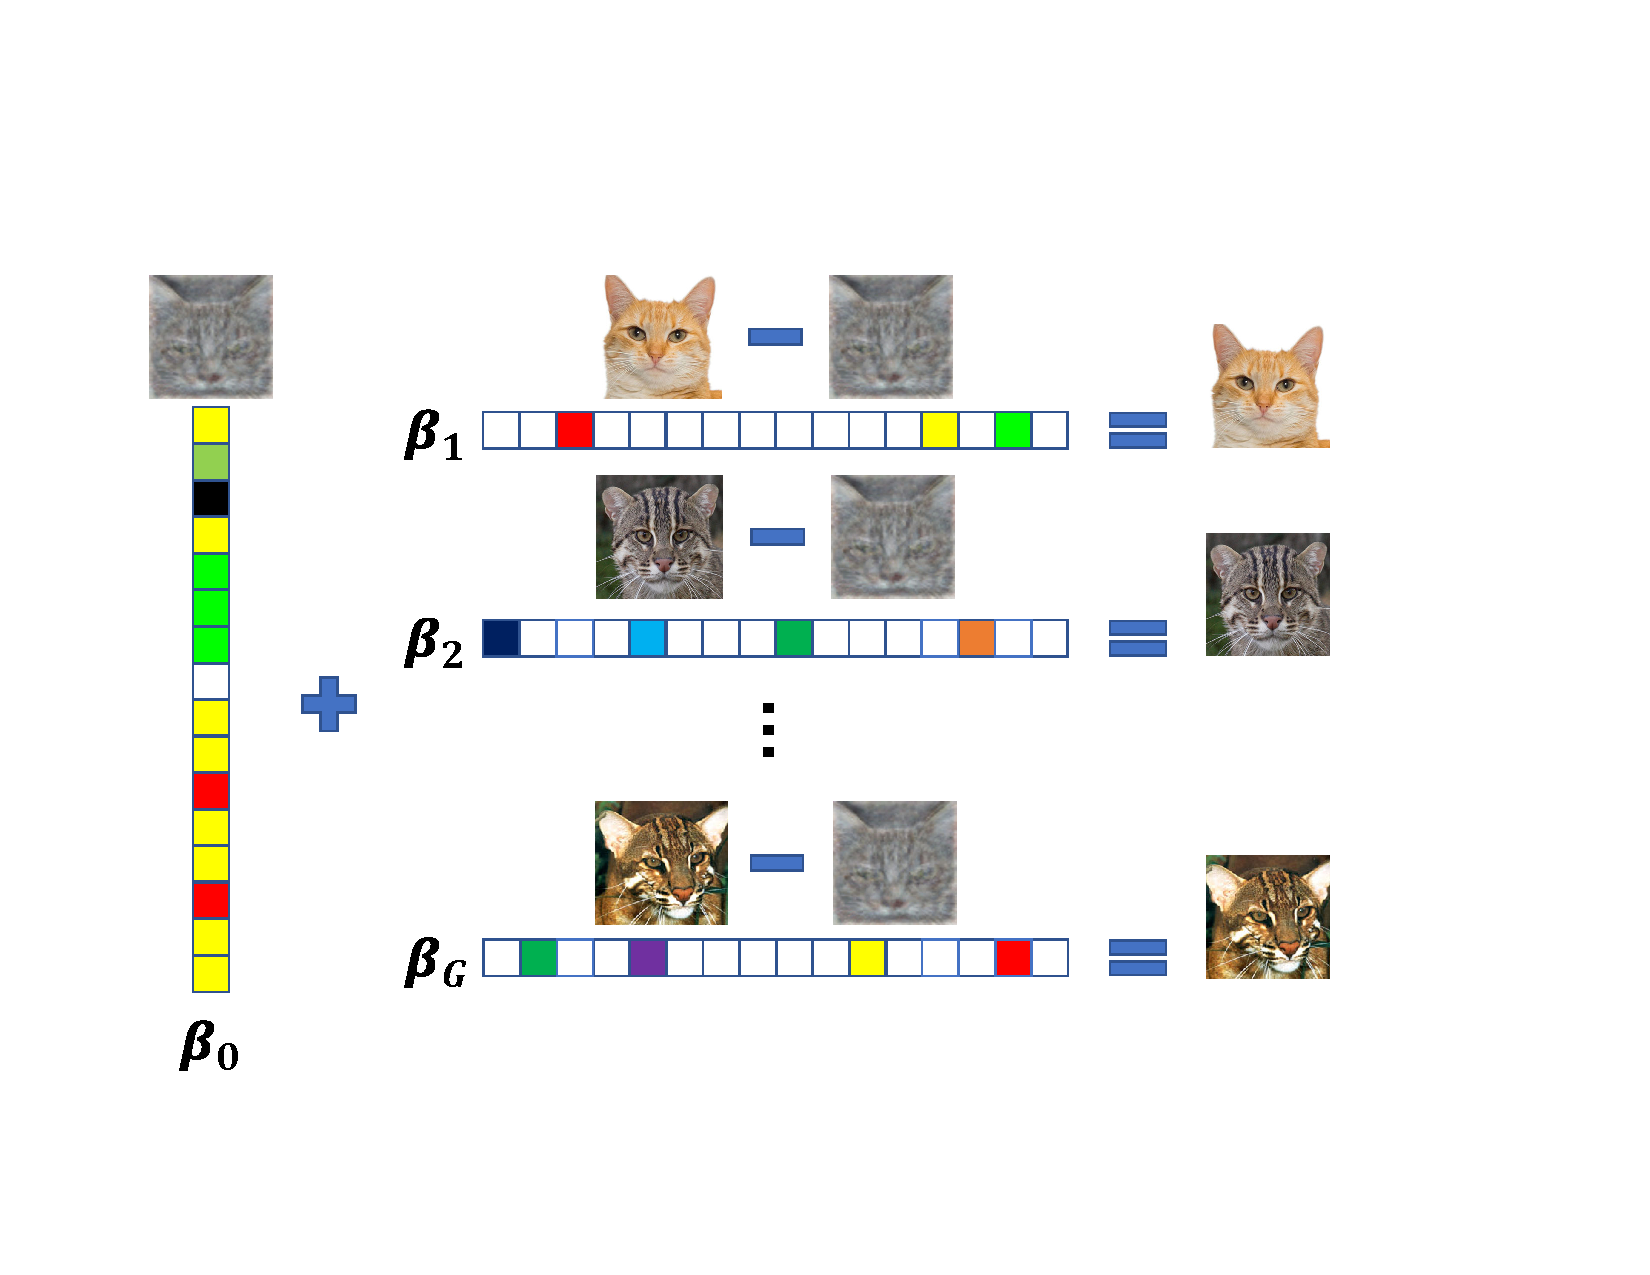
\includegraphics[scale=.25]{./img/concept.pdf}
%		\squeezeup
%		\caption{A conceptual illustration of data enrichment model for learning representation of  different cat species. The common parameter $\bbeta_0$ captures a \emph{generic cat} which consists of shared features among all cats.}
%		\label{fig:cat}		
%\end{figure}  
%{\bf Contributions:}
{\bf Notation and Preliminaries:}
We denote sets by curly $\cV$, matrices by bold capital $\V$, random variables by capital $V$, and vectors by small bold $\v$ letters.
We take $[G] = \{0, \dots, G\}$ and $[G]_\setminus = [G] \setminus \{0\}$.
%\ab{Can we use $[G]= \{1,\ldots,G\}$ and use $G \cup \{0\}$ in places where we need to include $\{0\}$? The notation will be more explicit and easier to follow.} 

Given $G$ groups and $n_g$ samples in each as $\{ \{\x_{gi}, y_{gi} \}_{i=1}^{n_g} \}_{g = 1}^G$, we can form the per group design matrix $\X_g \in \reals^{n_g \times p}$ and output vector $\y_g \in \reals ^{n_g}$.
The total number of samples is  $n = \sum_{g = 1}^{G} n_g$.
The data enriched model takes the following vector form:
\be
\label{eq:dirtymodel}
\y_g = \X_g (\bbeta _0^* + \bbeta _g^*) + \oomega_g,  \quad \forall g \in [G]_\setminus
\ee
where each row of $\X_g$ is $\x_{gi}^T$ and $\oomega_g^T = (\omega_{g1}, \dots, \omega_{gn_g})$ is the noise vector.
% are indexed with either a single number as $\v(i)$ or an index set $\cA$ as $\v_{\cA}$.
%Row $i$ of the matrix $\V$ is shown as $\v_i$ and $j$th element of the vector $\v$ is shown as $\v(j)$.
%The $(i,j)$th element of the matrix $\V$ is shown in three ways: $\V_{ij}$, $\v_i(j)$, or $v_{ij}$.
%Throughout the manuscript $c_i$ and $C_i$ are positive constants.
%We name the sample covariance of any matrix $M$ by $S_M$ vs. the actual parameter $\Sigma_M$.

%\noindent {\bf Sub-Gaussian (Sub-exponential) random variable and vector.}
A random variable $V$ is sub-Gaussian if its moments satisfies $\forall p \geq 1: (\ex |V|^p )^{1/p} \leq K_2 \sqrt{p}$.
The minimum value of $K_2$ is called the sub-Gaussian  norm of $V$, denoted by $\normth{V}{\psi_2}$ \cite{vers12}.
A random vector $\v \in \reals^p$ is sub-Gaussian if the one-dimensional marginals $\langle \v, \u \rangle$ are sub-Gaussian random variables for all $\u \in \reals^p$. The sub-Gaussian norm of $\v$ is defined \cite{vers12} as $\normth{\v}{\psi_2} = \sup_{\u \in \sphere} \normth{\langle \v, \u \rangle}{\psi_2}$.
%We abuse notation and use shorthand $\v \sim \subg(0, \Sigma_{\v}, K_{\v})$ for zero mean sub-Gaussian random vector with covariance $\Sigma_{\v}$ and sub-Gaussian norm of $K_{\v}$, although keeping in mind that no other moments, nor the exact form of the distribution function is known.
For any set $\cV \in \reals^p$ the Gaussian width of the set $\cV$ is defined as $\omega(\cV) = \ex_\g \left[ \sup_{\u \in \cV} \langle \g, \u \rangle \right]$ \cite{vershynin2018high}, where the expectation is over $\g \sim N(\0, \I_{p \times p})$, a vector of independent zero-mean unit-variance Gaussian.

%We define the minimum and maximum eigenvalues of a matrix $\M$ restricted to the set $\cA \subseteq \eS^{p-1}$ as $\lambda_{\min}(\M|\cA) = \inf_{\u \in \cA} \u^T \M \u$, and $\lambda_{\max}(\M|\cA) = \sup_{\u \in \cA} \u^T \M \u$ respectively.
%All $c_i$, $c$, and $C$ represent universal constants throughout the manuscript.
%Set $[G] = \{0, \dots, G\}$ is the index set for both shared and individual components (in the setting of data enriched model \eqref{eq:dsl}) and $[G]_\setminus = [G] - \{ 0 \}$ represents only the individual ones.


%\subsection{Contributions}
{\bf Contributions:}
We propose the following Data Enrichment (DE) estimator $\hbbe$ for recovering the structured parameters where the structure is induced by \emph{convex} functions $f_g(\cdot)$:
{\small\be
	\label{eq:super}
	\hbbe = (\hbbe_0^T, \dots, \hbbe_G^T) \in \argmin_{\bbeta _0, \dots, \bbeta _G} \frac{1}{n} \sum_{g=1}^{G} \norm{\y_g - \X_g (\bbeta _0 + \bbeta _g)}{2}^2,
	\\ \nr
	\text{s.t.} \quad \forall g \in [G]:f_g(\bbeta _g) \leq f_g(\bbeta _g^*).
\ee}
%We are investigating the conjecture that the pooled data from all groups will facilitate estimation of the common parameter $\bbeta_0^*$ in both samples complexity and error-bound rate regards.
%In our work, we explicitly answer these questions as follows:
We present several statistical and computational results for the DE estimator \eqref{eq:super} of the data enriched model:
\begin{itemize}[leftmargin = .4cm]
	\item The DE estimator \eqref{eq:super} succeeds if a geometric condition that we call \emph{Data EnRichment Incoherence Condition} (DERIC) is satisfied, Figure \ref{fig:deric}. Compared to other known geometric conditions in the literature such as structural coherence \cite{guba16} and stable recovery conditions \cite{mctr13}, DERIC is a weaker condition, Figure \ref{fig:sc}.
	\item Assuming DERIC holds, we establish a high probability non-asymptotic bound on the weighted sum of parameter-wise estimation error, $\ddelta_g = \hbbe_g - \bbeta_g^*$ as:
	\be
	\label{eq:errorsum}
	\sum_{g=0}^{G}  \sqrt{\frac{n_g}{n}} \|\ddelta_g\|_2 \leq  \gamma O\left(\frac{\max_{g \in [G]} \omega(\cC_g \cap \sphere)}{\sqrt{n}}\right),
%	\sum_{g=0}^{G}  \sqrt{\frac{n_g}{n}} \|\ddelta_g\|_2 \leq  C \gamma \frac{\max_{g \in [G]} \omega(\cC_g \cap \sphere) + \sqrt{\log (G+1)}}{\sqrt{n}},
	\ee
	where $n_0 \triangleq n$ is the total number of samples, $\gamma \triangleq \max_{g \in [G] } \frac{n}{n_g}$ is the \emph{sample condition number}, and $\cC_g$ is the error cone corresponding to $\bbeta_g^*$ exactly defined in Section \ref{sec:esti}.
	To the best of our knowledge, this is the first statistical estimation guarantee for the data enrichment.%ed model.
	%Gaussian width of a set $\cS$ is $\omega(\cS) = \ex_\g \left[ \sup_{\u \in \cS} \langle \g, \u \rangle \right]$. Gaussian width has been a standard tool for capturing the complexity of high-dimensional problems \cite{venkat12}.
	
%	Similar to previous works, we make a geometric assumption regarding the relation $\cC_g$s in each individual problem which is known as Structural Coherence assumption \cite{guba16, trop15}.
%	\item The general bound of \eqref{eq:errorsum} entails the following bounds for specific parameters:
%	\be
%	\nr
%	\forall g \in [G]: \norm{\ddelta_g}{2} \leq c \gamma \frac{\max_{g \in [G]} \omega(\cC_g \cap \sphere) + c\sqrt{\log G}}{\sqrt{n_g}}
%	\ee
%	Observe that $l_2$-norm of the estimation error for the common parameter decays as $1/\sqrt{n}$, similar to the well-studied high dimensional regression case \cite{venkat12, banerjee14}.
%	So the common parameter's estimator exploits all of the pooled data to reduce its error.
	\item We also establish the sample complexity of the DE estimator for all parameters as $\forall g \in [G]: n_g = O(\omega(\cC_g \cap \sphere))^2$. We emphasize that our result proofs that the recovery of the common parameter $\bbeta_0$ by DE estimator benefits from \emph{all} of the $n$ pooled samples.
	\item We present an efficient projected block gradient descent algorithm \emph{\dc}, to solve DE's objective \eqref{eq:super} which converges geometrically to the statistical error bound of \eqref{eq:errorsum}. To the best of our knowledge, this is the first rigorous computational result for the high-dimensional data-enriched regression.
%	\item We illustrate promising empirical performance of the model on synthetic data as well as on the problem of finding bio-markers associated with drug sensitivity of cell lines from different cancer types, where the support of estimated individual parameters $\text{supp}(\hbbe_g)$ for each cancer type $g$ represents a different set of bio-markers per cancer type.
\end{itemize}

%The rest of this paper is organized as follows:
%%First, we present a review of the related works in Section \ref{relwork}.
%First, we characterize the error set of our estimator and provide a deterministic error bound in Section \ref{sec:esti}.
%Then in Section \ref{sec:re}, we discuss the restricted eigenvalue condition and calculate the sample complexity required for the recovery of the true parameters by our estimator under DERIC condition.
%We close the statistical analysis in Section \ref{sec:error} by providing non-asymptotic high probability error bound for parameter recovery.
%We delineate our geometrically convergent algorithm, \dc{} in Section \ref{sec:opt} and finally supplement our work with synthetic and real experiments in Sections \ref{sec:expds} and \ref{realexp}.

\begin{figure}[t!]
	\centering
	\begin{subfigure}[t]{0.18\textwidth}
		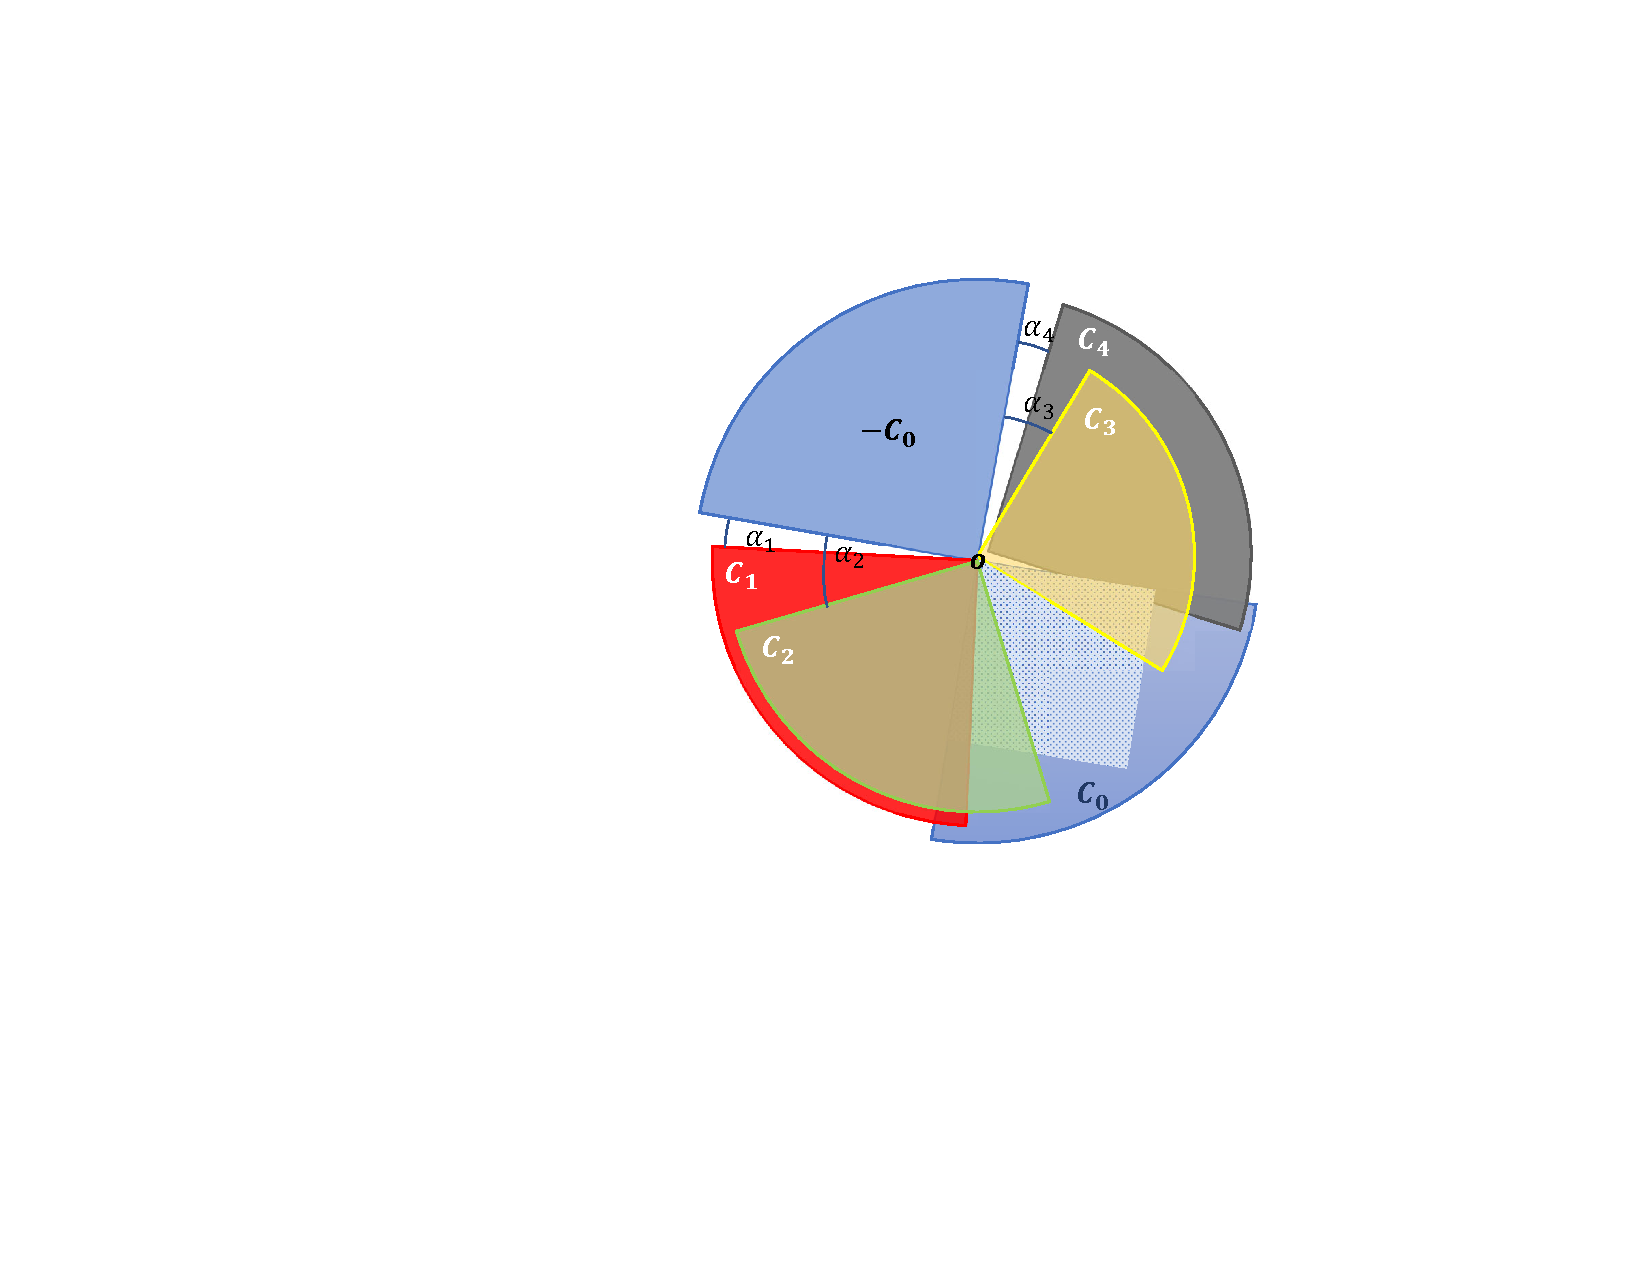
\includegraphics[width=\textwidth]{./img/sc.pdf}
		\caption{Structural Coherence (SC) condition.}\label{fig:sc}
	\end{subfigure} 
	~
	\begin{subfigure}[t]{0.18\textwidth}
		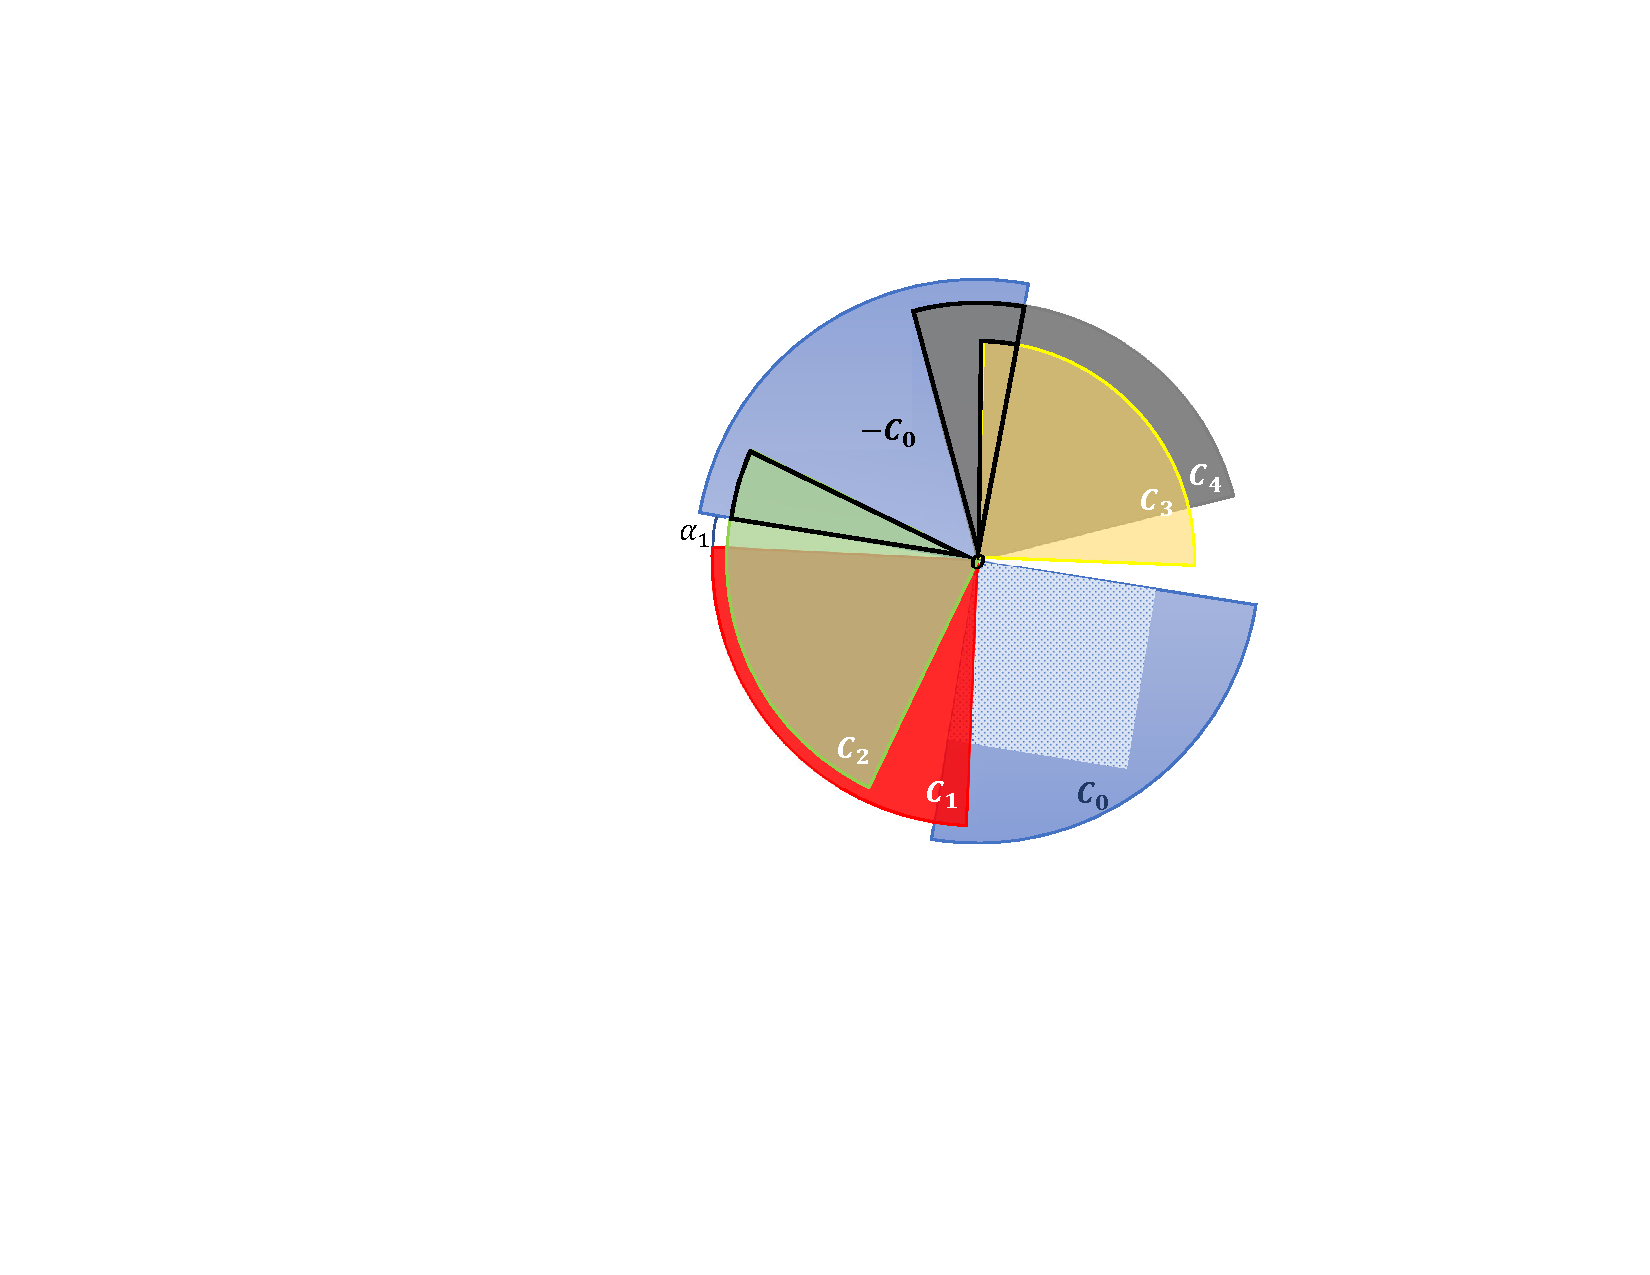
\includegraphics[width=1.04\textwidth]{./img/deric.pdf}
		\caption{Data EnRichment Incoherence Condition (DERIC). }
		\label{fig:deric}
	\end{subfigure}
	\squeezeup
	\caption{a) State of the art condition for recovering common and individual parameters in superposition models where $\cC_g = \text{Cone}(\cE_g)$ are error cones and $\cE_g = \left\{\ddelta_g | f_g(\bbeta _g^* + \ddelta_g) \leq f_g(\bbeta _g^*)\right\}$ are the error sets for each parameter $\bbeta^*_g \in [G]$ \cite{guba16} b) Our more relaxed recovery condition which allows \emph{arbitrary non-zero fraction } of the error cones of individual parameters intersect with $-\cC_0$.}
	\label{fig syn2}
\end{figure}




%In machine learning, limited training samples in many applications such as medicine has led to a collection of learning methods known as \emph{Multi-Task Learning} (MLT) \cite{Zhang2017-rm}. In supervised parametric setting such as regression, the relation between tasks is captured by explicitly modeling the relation between their parameters. One class of such modeling assumes that the parameter matrix 

